\hypertarget{domain-oriented-software-development-desc-method}{%
\section{Domain Oriented Software-Development -- DESC
Method}\label{domain-oriented-software-development-desc-method}}

An Embedded-System is a computer system, which works as part of a Technical-System.

\hypertarget{special-requirements}{%
\subsection{Special requirements}\label{special-requirements}}

\begin{itemize}
\tightlist
\item
  Reactive functionality

  \begin{itemize}
  \tightlist
  \item
    An Embedded-System has to react on external events
  \item
    Many events can happen at the same time
  \end{itemize}
\item
  Hard Real-time requirements

  \begin{itemize}
  \tightlist
  \item
    Has to react within a defined time
  \item
    Otherwise it is just unusable or it can even cause harm
  \end{itemize}
\item
  Reliability

  \begin{itemize}
  \tightlist
  \item
    May by safety critical
  \item
    Software-updates expensive
  \item
    Faults can cause material damage
  \end{itemize}
\item
  Economic efficiency

  \begin{itemize}
  \tightlist
  \item
    High number of units
  \item
    Power consumption
  \item
    Battery size
  \item
    Unit cost
  \end{itemize}
\item
  Extreme environmental conditions

  \begin{itemize}
  \tightlist
  \item
    Electromagnetic Compatibility (EMC), temperature, \ldots{}
  \end{itemize}
\item
  Product lines
\item
  Testability
\end{itemize}
\clearpage

\hypertarget{uml-introduction}{%
\subsection{UML Introduction}\label{uml-introduction}}

\hypertarget{relationships}{%
\subsubsection{Relationships}\label{relationships}}

We distinguish between Composition, Dependency as well as Association
and Aggregation\\

\textbf{Composition}:\\
\begin{itemize}
    \item Composition defines a whole-part relationship
    \item Describes how objects are composed of other objects
    \item Two possible Notations:
\end{itemize}

\begin{figure}[H]
\centering
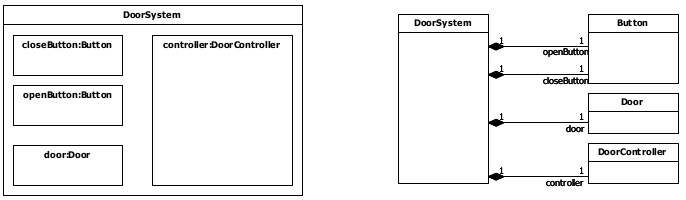
\includegraphics[width=0.7\textwidth]{figures/compositionUml.png}
\caption{UML Composition}
\end{figure}

\textbf{Direction:}\\
The composition can have a direction or is bidirectional:

\begin{figure}[H]
\centering
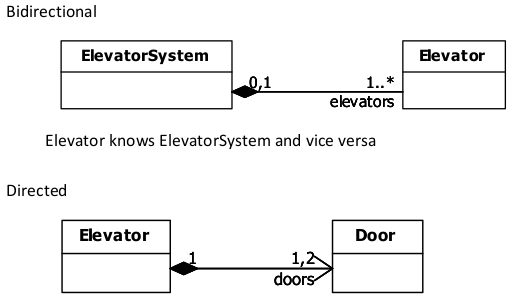
\includegraphics[width=0.5\textwidth]{figures/directionCompositionUml.png}
\caption{Navig-ability Composition}
\end{figure}

\textbf{Links:}\\
The dependency between two instances or objects are called links.

\hypertarget{association}{%
\paragraph{Association:}\label{association}}

Association is a relationship between classes. 

\begin{itemize}
    \item An instance of class A knows one or more instances of class B
    \item The instances of class B are referenced (NOT CONTAINED!)
    \item When an instance of A is deleted, the bs (involved instances of B) will not be deleted
    \item When an instance of A is copied, only the references to the bs will be copied. (shallow copy)
    \item (in undirected, bidirectional relationships, i.e.~without arrow, each referenced object has a corresponding back reference)
\end{itemize}

\begin{figure}[H]
\centering
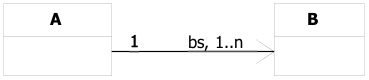
\includegraphics[width=0.4\textwidth]{figures/associationUml.png}
\caption{Association}
\end{figure}

\hypertarget{aggregation}{%
\paragraph{Aggregation}\label{aggregation}}

\begin{figure}[H]
\centering
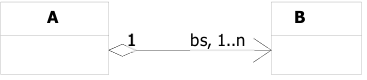
\includegraphics[width=0.5\textwidth]{figures/aggregtionUml.png}
\caption{Aggregation}
\end{figure}

\hypertarget{basic-terms-and-concepts}{%
\subsection{Basic Terms and Concepts}\label{basic-terms-and-concepts}}

\hypertarget{technical-processes}{%
\subsubsection{Technical-Processes}\label{technical-processes}}

\begin{tcolorbox}[colback=red!5!white,colframe=red!75!black]
Two Technical-Processes are parallel i.e.~sequentially independent, if their states are physically independent
\end{tcolorbox}

\textbf{Events:} 
\begin{itemize}
    \item Events are a consequence of a relevant state change of a Technical-Process
    \item Events can be defined as a transition of a Technical-Process from one discrete state to another
    \item Events may hold attributes
    \item Attributes may be any kind of additional information such as measurable quantities
\end{itemize}

\begin{lstlisting}
doorClosed(currentTime)
\end{lstlisting}


\textbf{Actions:} 
\begin{itemize}
    \item Actions are the means to control a Technical-Process i.e.~to have influence on it
    \item Examples of actions:
    \begin{itemize}
        \item motorOn, motorOff
        \item valveOpen, valveClose
    \end{itemize}
    \item An actions can indirectly cause a Technical-Process to change its state
    \item The effect of an action depends on the current state of the Technical-Process
\end{itemize}

\hypertarget{state-diagram-for-technical-processes}{%
\subsubsection{State-Diagram for
Technical-Processes}\label{state-diagram-for-technical-processes}}

\begin{figure}[H]
\centering
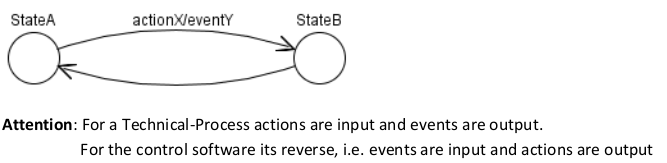
\includegraphics[width=0.6\textwidth]{figures/stateMachine.png}
\caption{State Machine}
\end{figure}

\hypertarget{key-concepts}{%
\subsection{Key Concepts}\label{key-concepts}}

\hypertarget{correspondence-principle}{%
\subsubsection{Correspondence
Principle}\label{correspondence-principle}}

The software structure of an embedded-system must correspond to the
structure and the behaviour of the technical-system.

\hypertarget{formal-model}{%
\subsubsection{Formal Model}\label{formal-model}}

\begin{itemize}
\tightlist
\item
  Basic requirement for the Correspondence Principle
\item
  A clear correspondence between program structure and real environment
  is almost impossible
\item
  The semantics of programing languages is not built for a
  correspondence on this level of abstraction
\item
  Enables code generation
\item
  To generate code, a model has to be formal and complete i.e.~all
  necessary information has to be contained in the model in a machine
  readable form
\item
  Model and code are always consistent
\end{itemize}

\hypertarget{component-architecture}{%
\subsubsection{Component Architecture}\label{component-architecture}}

\begin{itemize}
\tightlist
\item
  Model consists of components and connectors
\item
  Explicit connectors must be independent elements of a composition
\item
  Components have to fulfil the correspondence principle
\item
  Components of the real system are represented in the model by
  corresponding objects (Boundary-Objects)
\end{itemize}

\hypertarget{separation-of-concerns}{%
\subsubsection{Separation of Concerns}\label{separation-of-concerns}}

\textbf{Separation of the problem areas}

Control Software (Control) 
\begin{itemize}
    \item Realisation of the functional requirements
    \item Depends only on the functional requirements and the Technical-Processes
\end{itemize}

Connection Software (Connection)
\begin{itemize}
    \item Connection between control software and computer interfaces
    \item Implements the so called Virtual Interaction (see below)
\end{itemize}

Execution Software (Execution) 
\begin{itemize}
    \item Control and connection software are passive parts of the Embedded-System
    \item Execution Software is the active part of the Embedded-System software
    \item Activates control and connection
    \item Is responsible for meeting the timing requirements
\end{itemize} 

This decomposition into three problem areas is supported by the
following concepts: 
\begin{itemize}
    \item Generic Software Architecture (see below)
    \item Virtual Interaction (see below)
\end{itemize}

\hypertarget{generic-software-architecture-control}{%
\subsubsection{Generic Software Architecture
(Control)}\label{generic-software-architecture-control}}

red = Control, blue=Connection, green = Execution

The \textbf{Technical Process} is something physical, like the process
of a coffee mashine.\\
\textbf{This picture is important! We need this in our summary, the
lecturer said.}

\begin{figure}[H]
\centering
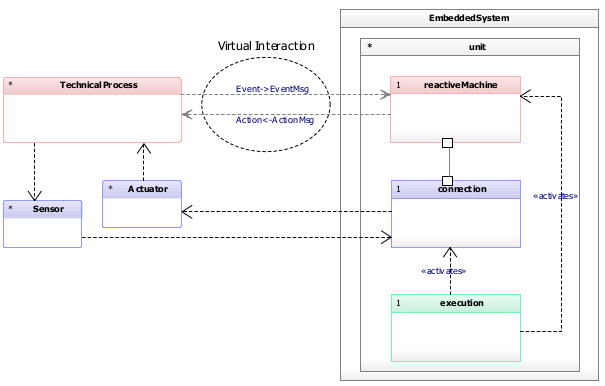
\includegraphics[width=0.8\textwidth]{figures/genericSoftwareArchitecture.png}
\caption{Generic Software Architecture}
\end{figure}

\textbf{reactiveMachine}\\
Reacts on inputs and generates outputs. - Reactive-Machine (RM) works
sequentially (Queue) - Handling of an Event cannot be interrupted by
other Event-Messages

\hypertarget{virtual-interaction-connection}{%
\subsubsection{Virtual Interaction
(Connection)}\label{virtual-interaction-connection}}

\begin{figure}[H]
\centering
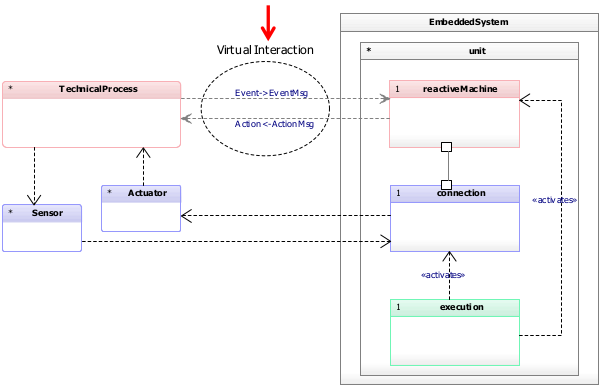
\includegraphics[width=0.8\textwidth]{figures/virtualInteraction.png}
\caption{Virtual Interaction}
\end{figure}

The interaction between the technical process and the reactive Machine
is just virtual.\\
e.g.~In a Technical-Process the event highTemp occurs, the
Reactive-Machine receives an equally named Event-Message.

The connection is the implementation of this virtual interaction. 
\begin{itemize}
    \item It reads the input-signals from ports or any other interface
    \item Detects Events
    \item  Generates Event-Messages
    \item Writes Event-Messages into a message buffer (e.g.~queue)
    \item Generates output
\end{itemize}

\hypertarget{execution}{%
\subsubsection{Execution}\label{execution}}

\emph{Somehow the main loop of this unit.}

\begin{itemize}
\tightlist
\item
  Controls the sequence of activation of the passive parts of the unit
\item
  Responsible for

  \begin{itemize}
  \tightlist
  \item
    Management of input- and output-message buffer (queue)
  \item
    Scheduling
  \end{itemize}
\end{itemize}

\hypertarget{summary}{%
\subsection{Summary}\label{summary}}

\begin{figure}[H]
\centering
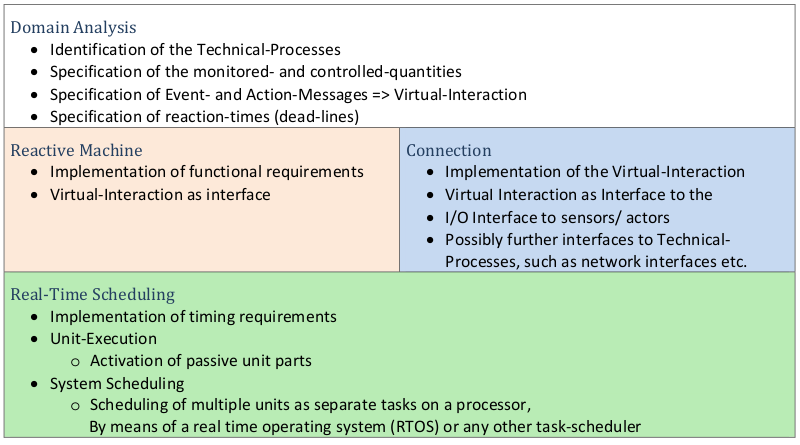
\includegraphics[width=1\textwidth]{figures/summaryDesc.png}
\caption{Summary of Desc}
\end{figure}

\clearpage